\documentclass[sigconf]{acmart}


\IfFileExists{upquote.sty}{\usepackage{upquote}}{}
\IfFileExists{microtype.sty}{% use microtype if available
  \usepackage[]{microtype}
  \UseMicrotypeSet[protrusion]{basicmath} % disable protrusion for tt fonts
}{}
\makeatletter
\@ifundefined{KOMAClassName}{% if non-KOMA class
  \IfFileExists{parskip.sty}{%
    \usepackage{parskip}
  }{% else
    \setlength{\parindent}{0pt}
    \setlength{\parskip}{6pt plus 2pt minus 1pt}}
}{% if KOMA class
  \KOMAoptions{parskip=half}}
\makeatother

%%
%% This is file `sample-manuscript.tex',
%% generated with the docstrip utility.
%%
%% The original source files were:
%%
%% samples.dtx  (with options: `manuscript')
%% 
%% IMPORTANT NOTICE:
%% 
%% For the copyright see the source file.
%% 
%% Any modified versions of this file must be renamed
%% with new filenames distinct from sample-manuscript.tex.
%% 
%% For distribution of the original source see the terms
%% for copying and modification in the file samples.dtx.
%% 
%% This generated file may be distributed as long as the
%% original source files, as listed above, are part of the
%% same distribution. (The sources need not necessarily be
%% in the same archive or directory.)
%%
%%
%% Commands for TeXCount
%TC:macro \cite [option:text,text]
%TC:macro \citep [option:text,text]
%TC:macro \citet [option:text,text]
%TC:envir table 0 1
%TC:envir table* 0 1
%TC:envir tabular [ignore] word
%TC:envir displaymath 0 word
%TC:envir math 0 word
%TC:envir comment 0 0
%%
%%
%% The first command in your LaTeX source must be the \documentclass command.


% Options for packages loaded elsewhere
\PassOptionsToPackage{unicode}{hyperref}
\PassOptionsToPackage{hyphens}{url}
\PassOptionsToPackage{dvipsnames,svgnames,x11names}{xcolor}

\IfFileExists{bookmark.sty}{\usepackage{bookmark}}{\usepackage{hyperref}}

%% PANDOC PREAMBLE BEGINS

\usepackage{longtable,booktabs,array}
\newcounter{none} % for unnumbered tables
\usepackage{calc} % for calculating minipage widths
% Correct order of tables after \paragraph or \subparagraph
\usepackage{etoolbox}
\makeatletter
\patchcmd\longtable{\par}{\if@noskipsec\mbox{}\fi\par}{}{}
\makeatother
% Allow footnotes in longtable head/foot
\IfFileExists{footnotehyper.sty}{\usepackage{footnotehyper}}{\usepackage{footnote}}
\makesavenoteenv{longtable}
\usepackage{graphicx}
\makeatletter
\newsavebox\pandoc@box
\newcommand*\pandocbounded[1]{% scales image to fit in text height/width
  \sbox\pandoc@box{#1}%
  \Gscale@div\@tempa{\textheight}{\dimexpr\ht\pandoc@box+\dp\pandoc@box\relax}%
  \Gscale@div\@tempb{\linewidth}{\wd\pandoc@box}%
  \ifdim\@tempb\p@<\@tempa\p@\let\@tempa\@tempb\fi% select the smaller of both
  \ifdim\@tempa\p@<\p@\scalebox{\@tempa}{\usebox\pandoc@box}%
  \else\usebox{\pandoc@box}%
  \fi%
}
% Set default figure placement to htbp
\def\fps@figure{htbp}
\makeatother





\setlength{\emergencystretch}{3em} % prevent overfull lines

\providecommand{\tightlist}{%
  \setlength{\itemsep}{0pt}\setlength{\parskip}{0pt}}





\usepackage{booktabs}
\usepackage{longtable}
\usepackage{array}
\usepackage{multirow}
\usepackage{wrapfig}
\usepackage{float}
\usepackage{colortbl}
\usepackage{pdflscape}
\usepackage{tabu}
\usepackage{threeparttable}
\usepackage{threeparttablex}
\usepackage[normalem]{ulem}
\usepackage{makecell}
\usepackage{xcolor}
\usepackage{tcolorbox}
\definecolor{mypink}{RGB}{219, 48, 122}
\makeatletter
\@ifpackageloaded{caption}{}{\usepackage{caption}}
\AtBeginDocument{%
\ifdefined\contentsname
  \renewcommand*\contentsname{Table of contents}
\else
  \newcommand\contentsname{Table of contents}
\fi
\ifdefined\listfigurename
  \renewcommand*\listfigurename{List of Figures}
\else
  \newcommand\listfigurename{List of Figures}
\fi
\ifdefined\listtablename
  \renewcommand*\listtablename{List of Tables}
\else
  \newcommand\listtablename{List of Tables}
\fi
\ifdefined\figurename
  \renewcommand*\figurename{Figure}
\else
  \newcommand\figurename{Figure}
\fi
\ifdefined\tablename
  \renewcommand*\tablename{Table}
\else
  \newcommand\tablename{Table}
\fi
}
\@ifpackageloaded{float}{}{\usepackage{float}}
\floatstyle{ruled}
\@ifundefined{c@chapter}{\newfloat{codelisting}{h}{lop}}{\newfloat{codelisting}{h}{lop}[chapter]}
\floatname{codelisting}{Listing}
\newcommand*\listoflistings{\listof{codelisting}{List of Listings}}
\makeatother
\makeatletter
\makeatother
\makeatletter
\@ifpackageloaded{caption}{}{\usepackage{caption}}
\@ifpackageloaded{subcaption}{}{\usepackage{subcaption}}
\makeatother
%% PANDOC PREAMBLE ENDS

\setlength{\parindent}{10pt}
\setlength{\parskip}{0pt}

\hypersetup{
  pdftitle={Donation Behaviour in an Online Visualisation Experiment},
  pdfauthor={Gabriel Strain; Aaditya Mehrotra; Caroline Jay; Paul A. Warren; Andrew J. Stewart},
  colorlinks=true,
  linkcolor={blue},
  filecolor={Maroon},
  citecolor={Blue},
  urlcolor={red},
  pdfcreator={LaTeX via pandoc, via quarto}}

%% \BibTeX command to typeset BibTeX logo in the docs
\AtBeginDocument{%
  \providecommand\BibTeX{{%
    Bib\TeX}}}

%% Rights management information.  This information is sent to you
%% when you complete the rights form.  These commands have SAMPLE
%% values in them; it is your responsibility as an author to replace
%% the commands and values with those provided to you when you
%% complete the rights form.
\setcopyright{cc}
\copyrightyear{2027}
\acmYear{2027}
\acmDOI{10.1145/3706598.3713809}

%% These commands are for a PROCEEDINGS abstract or paper.
\acmConference[CHI'27]{CHI Conference on Human Factors in Computing
Systems}{April 26-May 1, 2027}{Pittsburgh, USA}
\acmPrice{}
%%
%%  Uncomment \acmBooktitle if the title of the proceedings is different
%%  from ``Proceedings of ...''!
%%

\acmISBN{}

%% Submission ID.
%% Use this when submitting an article to a sponsored event. You'll
%% receive a unique submission ID from the organizers
%% of the event, and this ID should be used as the parameter to this command.


%%
%% For managing citations, it is recommended to use bibliography
%% files in BibTeX format.
%%
%% You can then either use BibTeX with the ACM-Reference-Format style,
%% or BibLaTeX with the acmnumeric or acmauthoryear sytles, that include
%% support for advanced citation of software artefact from the
%% biblatex-software package, also separately available on CTAN.
%%
%% Look at the sample-*-biblatex.tex files for templates showcasing
%% the biblatex styles.
%%

%%
%% The majority of ACM publications use numbered citations and
%% references.  The command \citestyle{authoryear} switches to the
%% "author year" style.
%%
%% If you are preparing content for an event
%% sponsored by ACM SIGGRAPH, you must use the "author year" style of
%% citations and references.
%% Uncommenting
%% the next command will enable that style.
%%\citestyle{acmauthoryear}



%% end of the preamble, start of the body of the document source.
\begin{document}


%%
%% The "title" command has an optional parameter,
%% allowing the author to define a "short title" to be used in page headers.
\title{Donation Behaviour in an Online Visualisation Experiment}

%%
%% The "author" command and its associated commands are used to define
%% the authors and their affiliations.
%% Of note is the shared affiliation of the first two authors, and the
%% "authornote" and "authornotemark" commands
%% used to denote shared contribution to the research.


  \author{Gabriel Strain}
  \orcid{0000-0002-4769-9221}
            \affiliation{%
                  \institution{Department of Computer Science, Faculty
of Science and Engineering, University of Manchester}
                          \streetaddress{Oxford Road}
                          \city{Manchester}
                                  \country{United Kingdom}
                          \postcode{M13 9PL}
              }
        \author{Aaditya Mehrotra}
  \orcid{XX}
            \affiliation{%
                  \institution{Department of Computer Science, Faculty
of Science and Engineering, University of Manchester}
                          \streetaddress{Oxford Road}
                          \city{Manchester}
                                  \country{United Kingdom}
                          \postcode{M13 9PL}
              }
        \author{Caroline Jay}
  
            \affiliation{%
                  \institution{Department of Computer Science, Faculty
of Science and Engineering, University of Manchester}
                          \streetaddress{Oxford Road}
                          \city{Manchester}
                                  \country{United Kingdom}
                          \postcode{M13 9PL}
              }
        \author{Paul A. Warren}
  
            \affiliation{%
                  \institution{Division of Psychology, Communication and
Human Neuroscience, School of Health Sciences, Faculty of Biology,
Medicine, and Health, University of Manchester}
                          \streetaddress{Oxford Road}
                          \city{Manchester}
                                  \country{United Kingdom}
                          \postcode{M13 9PL}
              }
        \author{Andrew J. Stewart}
  
            \affiliation{%
                  \institution{Department of Computer Science, Faculty
of Science and Engineering, University of Manchester}
                          \streetaddress{Oxford Road}
                          \city{Manchester}
                                  \country{United Kingdom}
                          \postcode{M13 9PL}
              }
      
%% By default, the full list of authors will be used in the page
%% headers. Often, this list is too long, and will overlap
%% other information printed in the page headers. This command allows
%% the author to define a more concise list
%% of authors' names for this purpose.
%\renewcommand{\shortauthors}{Trovato et al.}
\renewcommand{\shortauthors}{Strain et al.}

%%  
%% The abstract is a short summary of the work to be presented in the
%% article.
\begin{abstract}
abstract goes here.    
\end{abstract}

%%
%% The code below is generated by the tool at http://dl.acm.org/ccs.cfm.
%% Please copy and paste the code instead of the example below.
%%
\begin{CCSXML}
<ccs2012>
 <concept>
  <concept_id>10003120.10003145</concept_id>
  <concept_desc>Human-centered computing~Visualization</concept_desc>
  <concept_significance>500</concept_significance>
 </concept>
 <concept>
  <concept_id>10003120.10003145.10011769</concept_id>
  <concept_desc>Human-centered computing~Empirical studies in visualization</concept_desc>
  <concept_significance>500</concept_significance>
 </concept>
 <concept>
  <concept_id>10003120.10003145.10011770</concept_id>
  <concept_desc>Human-centered computing~Visualization design and evaluation methods</concept_desc>
  <concept_significance>300</concept_significance>
 </concept>
 <concept>
  <concept_id>10003120.10003121.10011748</concept_id
  <concept_desc>Human-centered computing~Empirical studies in HCI</concept_desc>
  <concept_significance>500</concept_significance>
 </concept>
</ccs2012>
\end{CCSXML}

\ccsdesc[500]{Human-centered computing~Visualization}
\ccsdesc[500]{Human-centered computing~Empirical studies in visualization}
\ccsdesc[300]{Human-centered computing~Visualization design and evaluation methods}
\ccsdesc[500]{Human-centered computing~Empirical studies in HCI}

%%
%% Keywords. The author(s) should pick words that accurately describe
%% the work being presented. Separate the keywords with commas.
\keywords{donation behaviour, scatterplot, crowdsourced}


%%
%% This command processes the author and affiliation and title
%% information and builds the first part of the formatted document.
\maketitle

\setlength{\parskip}{-0.1pt}

\section{Introduction}\label{sec-intro}

\begin{itemize}
\tightlist
\item
  some justification for only using scatterplots
\item
  motivate the study of data visualisation and behaviour change
\item
  motivate the use of novel visualisation techniques
\item
\end{itemize}

\section{Related Work}\label{sec-related-work}

\subsection{Donation Behaviour}\label{sec-donation-behaviour}

\begin{itemize}
\tightlist
\item
  factors influencing charitable donations
\item
  specifically regarding online infographics/donation campaigns
\item
  do people donate more to things they like more?
\item
  do they donate more to things that show better outcomes?
\end{itemize}

\subsection{Behaviour and Data
Visualisation}\label{sec-behaviour-data-viz}

\begin{itemize}
\tightlist
\item
  how can data visualisation change people's behaviours?
\item
  the persuasive power of data visualisation and how can this extend to
  driving behaviour change
\item
  data visualisation and belief change
\item
  then, can this meaningfully be extended to modify behaviour?
\end{itemize}

\subsection{Correlation Perception \& Modified
Scatterplots}\label{sec-corr-percept}

\begin{itemize}
\tightlist
\item
  factors influencing correlation perception, including what we have
  found
\item
  how have scatterplots been modified to induce changes in correlation
  perception
\item
  then, how this has been shown to extend to belief change
\item
  motivate the study of behaviour change as a result of visualisation
  viewing
\item
  particularly, highlight the potential moral benefit of motivating
  better behaviour
\end{itemize}

\subsection{Using Visualisation Techniques to Drive Behaviour
Modification}\label{using-visualisation-techniques-to-drive-behaviour-modification}

\begin{itemize}
\tightlist
\item
  has anything like this been tested before? (I am assuming not)
\item
  hat are the potential implications of this?
\end{itemize}

\section{Hypotheses}\label{sec-hypotheses}

We formulate the first hypothesis based on previous evidence that people
will donate more money to charitable concerns that they prefer:

\begin{itemize}
\tightlist
\item
  H\textsubscript{1}: participants will donate more money to charities
  that they prefer, as tested by Likert scales and a charity ranking.
\end{itemize}

Owing to evidence that strong relationships portrayed in scatterplots
can induce belief change in viewers, and that, featured in data
visualisations can have effects on viewers' thoughts and attitudes, we
formulate the second hypothesis:

\begin{itemize}
\tightlist
\item
  H\textsubscript{2}: participants will donate more money to charities
  whose infographics feature scatterplots with higher \emph{r} values.
\end{itemize}

Finally, in light of evidence that scatterplots whose points have been
modified in such a way that correlation is perceived as higher and is
able to induce belief change to a greater degree, we formulate the third
hypothesis. This hypothesis is non-directional due to small effects
sizes reported in a previous study that utilised these techniques:

\begin{itemize}
\tightlist
\item
  H\textsubscript{3}: participants' donation amounts will be affected
  (non-directionally) by the type (standard or alternative) of
  scatterplot displayed.
\end{itemize}

\section{Methodology}\label{sec-methods}

In this section we begin by discussing our research methods, including
the open and reproducible research practices we used and the modelling
paradigms utilised in our analyses. We then detail the design of our
stimuli, the design of the experiment, the experimental procedure, and
participant recruitment and characteristics.

\subsection{Open Research}\label{sec-open-research}

The experiment was conducted according the principles of open and
reproducible research \citep{ayris_2018}. Hypotheses and analysis plans
were pre-registered with the Open Science Framework (OSF)\footnote{https://osf.io/kywt9/overview?view\_only=1f677775eb80467dae61c7502bc3305f}.
All data and analysis code are included in a GitHub
repository\footnote{removed for anon}, which also contains instructions
for building a Docker container \citep{merkel_2014} that reproduces the
computational environment in which the paper was written. By capturing
package versions and dependencies using the \texttt{renv} package
\citep{ushey_2026} in R, this container allows for full replication of
all stimuli, figures, analyses, and the paper itself. Ethical approval
was granted by \emph{removed for anon}.

\subsection{Modelling}\label{sec-modelling}

\subsection{Stimuli}\label{sec-stimuli}

\subsubsection{Charities}\label{sec-stimuli-charities}

Three charitable concerns were chosen for the experiment. Initially, we
intended to use the five charitable concerns outline in She and Sanfey,
2023 \citep{she_2023}. These were:

\begin{enumerate}
\def\labelenumi{\arabic{enumi}.}
\tightlist
\item
  Dog Rescue/Re-housing.
\item
  Environmental Protection.
\item
  Mental Health Helpline.
\item
  Education in Disadvantaged Communities.
\item
  Support for Homeless Individuals.
\end{enumerate}

Due to our inclusion of different correlations and scatterplot types,
the use of five charity categories would have resulted in an unfeasibly
large number of experimental trials. Concerns about participant fatigue
and experimental length led us to use only the first three charity
categories for the present experiment. After deciding on the three
charity categories, one author created candidate fictional charities for
each. Two authors then decided on a single fictional charity for each
category. Table~\ref{tbl-candidate-charities} shows the candidate
charities for each charity category. The final chosen charity is
highlighted in each case.

\begin{table}

\caption{\label{tbl-candidate-charities}The three chosen charity
categories, along with the candidate fictional charities for each. The
final chosen charity for each category is marked in bold and with an
asterisk in each case.}

\centering{

\begin{tabular}[t]{lll}
\toprule
Dog Rescue \& Re-housing & Environmental Protection & Mental Health Helpline\\
\midrule
West England Dog Re-Homing Centre & Welsh River Cleanup & SpeakUp\\
\textbf{Great British Dog Foundation*} & \textbf{Action for a Greener World*} & \textbf{Good Samaritans*}\\
London Dog’s Trust & British Bird’s Trust & Listen UK\\
\bottomrule
\end{tabular}

}

\end{table}%

\subsubsection{Charity Templates}\label{sec-stimuli-charity-templates}

\subsubsection{Scatterplot
Visualisations}\label{sec-stimuli-visualisations}

\subsection{Design}\label{sec-design}

We employed a fully within-subjects design. With 18 unique plots (3
charities \(\times\) 3 correlation values \(\times\) 2 plot types), all
unique combinations would result in \(\binom{18}{2} = 153\) pairs. To
decrease the task load on participants, we removed the 45 trials which
featured the same charity for a final total of 108 experimental trials.
Participants viewed all 108 experimental trials along with 6 attention
check trials, in a fully-randomised order. Our dependent variable was
the amount of money participants assigned to the left and right charity
infographics on a per-trial basis. The experiment, including all
stimuli, materials, and instructions, are hosted on GitLab
\href{The\%20pre-registration\%20states\%20that\%20150\%20participants\%20would\%20be\%20recruited.\%20Additional\%20participants\%20were\%20recruited\%20due\%20to\%20an\%20oversight,\%20however\%20all\%20conclusions\%20and\%20statistical\%20results\%20are\%20identical\%20when\%20run\%20with\%20164\%20or\%20150\%20participants.}{1\^{}}.

\subsection{Procedure}\label{sec-procedure}

The experiment was built using PsychoPy \citep{pierce_2019} and is
hosted on Pavlovia.org. Participants were instructed to only complete
the experiment on desktop or laptop computers. Each participants first
viewed the participant information sheet and provided consent by
checking boxes next to consent statements. Consent was required in order
to progress through the experiment. They were asked to provide their age
in a free text box, followed by their gender identity. Using Likert
scales, participants were then asked to indicate how important the three
chosen charitable concerns were to them (Dog Rescue and Re-Housing,
Environmental Protection, and Mental Health Helpline). Each Likert scale
featured seven points, and was anchored at points 1 and 7 with ``Not at
all important'' and ``Extremely important''. Participants then used a
drag-and-drop interface to rank the three charitable concerns. Following
the pre-experimental tests, participants were then asked to complete
eight rounds of the Remote Associated Test (RAT), which acted as a
filler task to prevent carryover effects \citep{she_2023}. Participants
were given 15 seconds for each round of the RAT, and were not required
to answer. Participants were given instructions, including the
following:

\hspace{0pt}
\begin{tcolorbox}[colback=gray!10, colframe=gray!50, boxrule=0.5pt]
...
\newline
  5. We encourage you to make assignments as if it were your own money.
  \newline
  6. To help you get into this mindset, the research team have decided to donate money to real-life charities based on the totals donated by all participants over the course of the experiment.
  \newline
  7. Once the experiment has concluded, you will receive an email detailing how the research team have split the money and which charities have been donated to.
  \newline
  ...
\end{tcolorbox}
\hspace{0pt}

Participants were informed that this was a deception at the conclusion
of the experiment. Following instructions, the experiment began. In a
series of 108 experimental trials, participants were asked to split 100
dollars between two charity infographics. Presentation order was
randomised, including 6 attention check trials which explicitly asked
participants to assign 100 dollars to either the left (n = 3) or the
right (n = 3) charity infographic. An example of an experimental trial
can be seen in Figure~\ref{fig-example-trial}. After completing all
trials, participants were debriefed regarding the deception employed and
thanked for their participation.

\begin{figure*}

\centering{

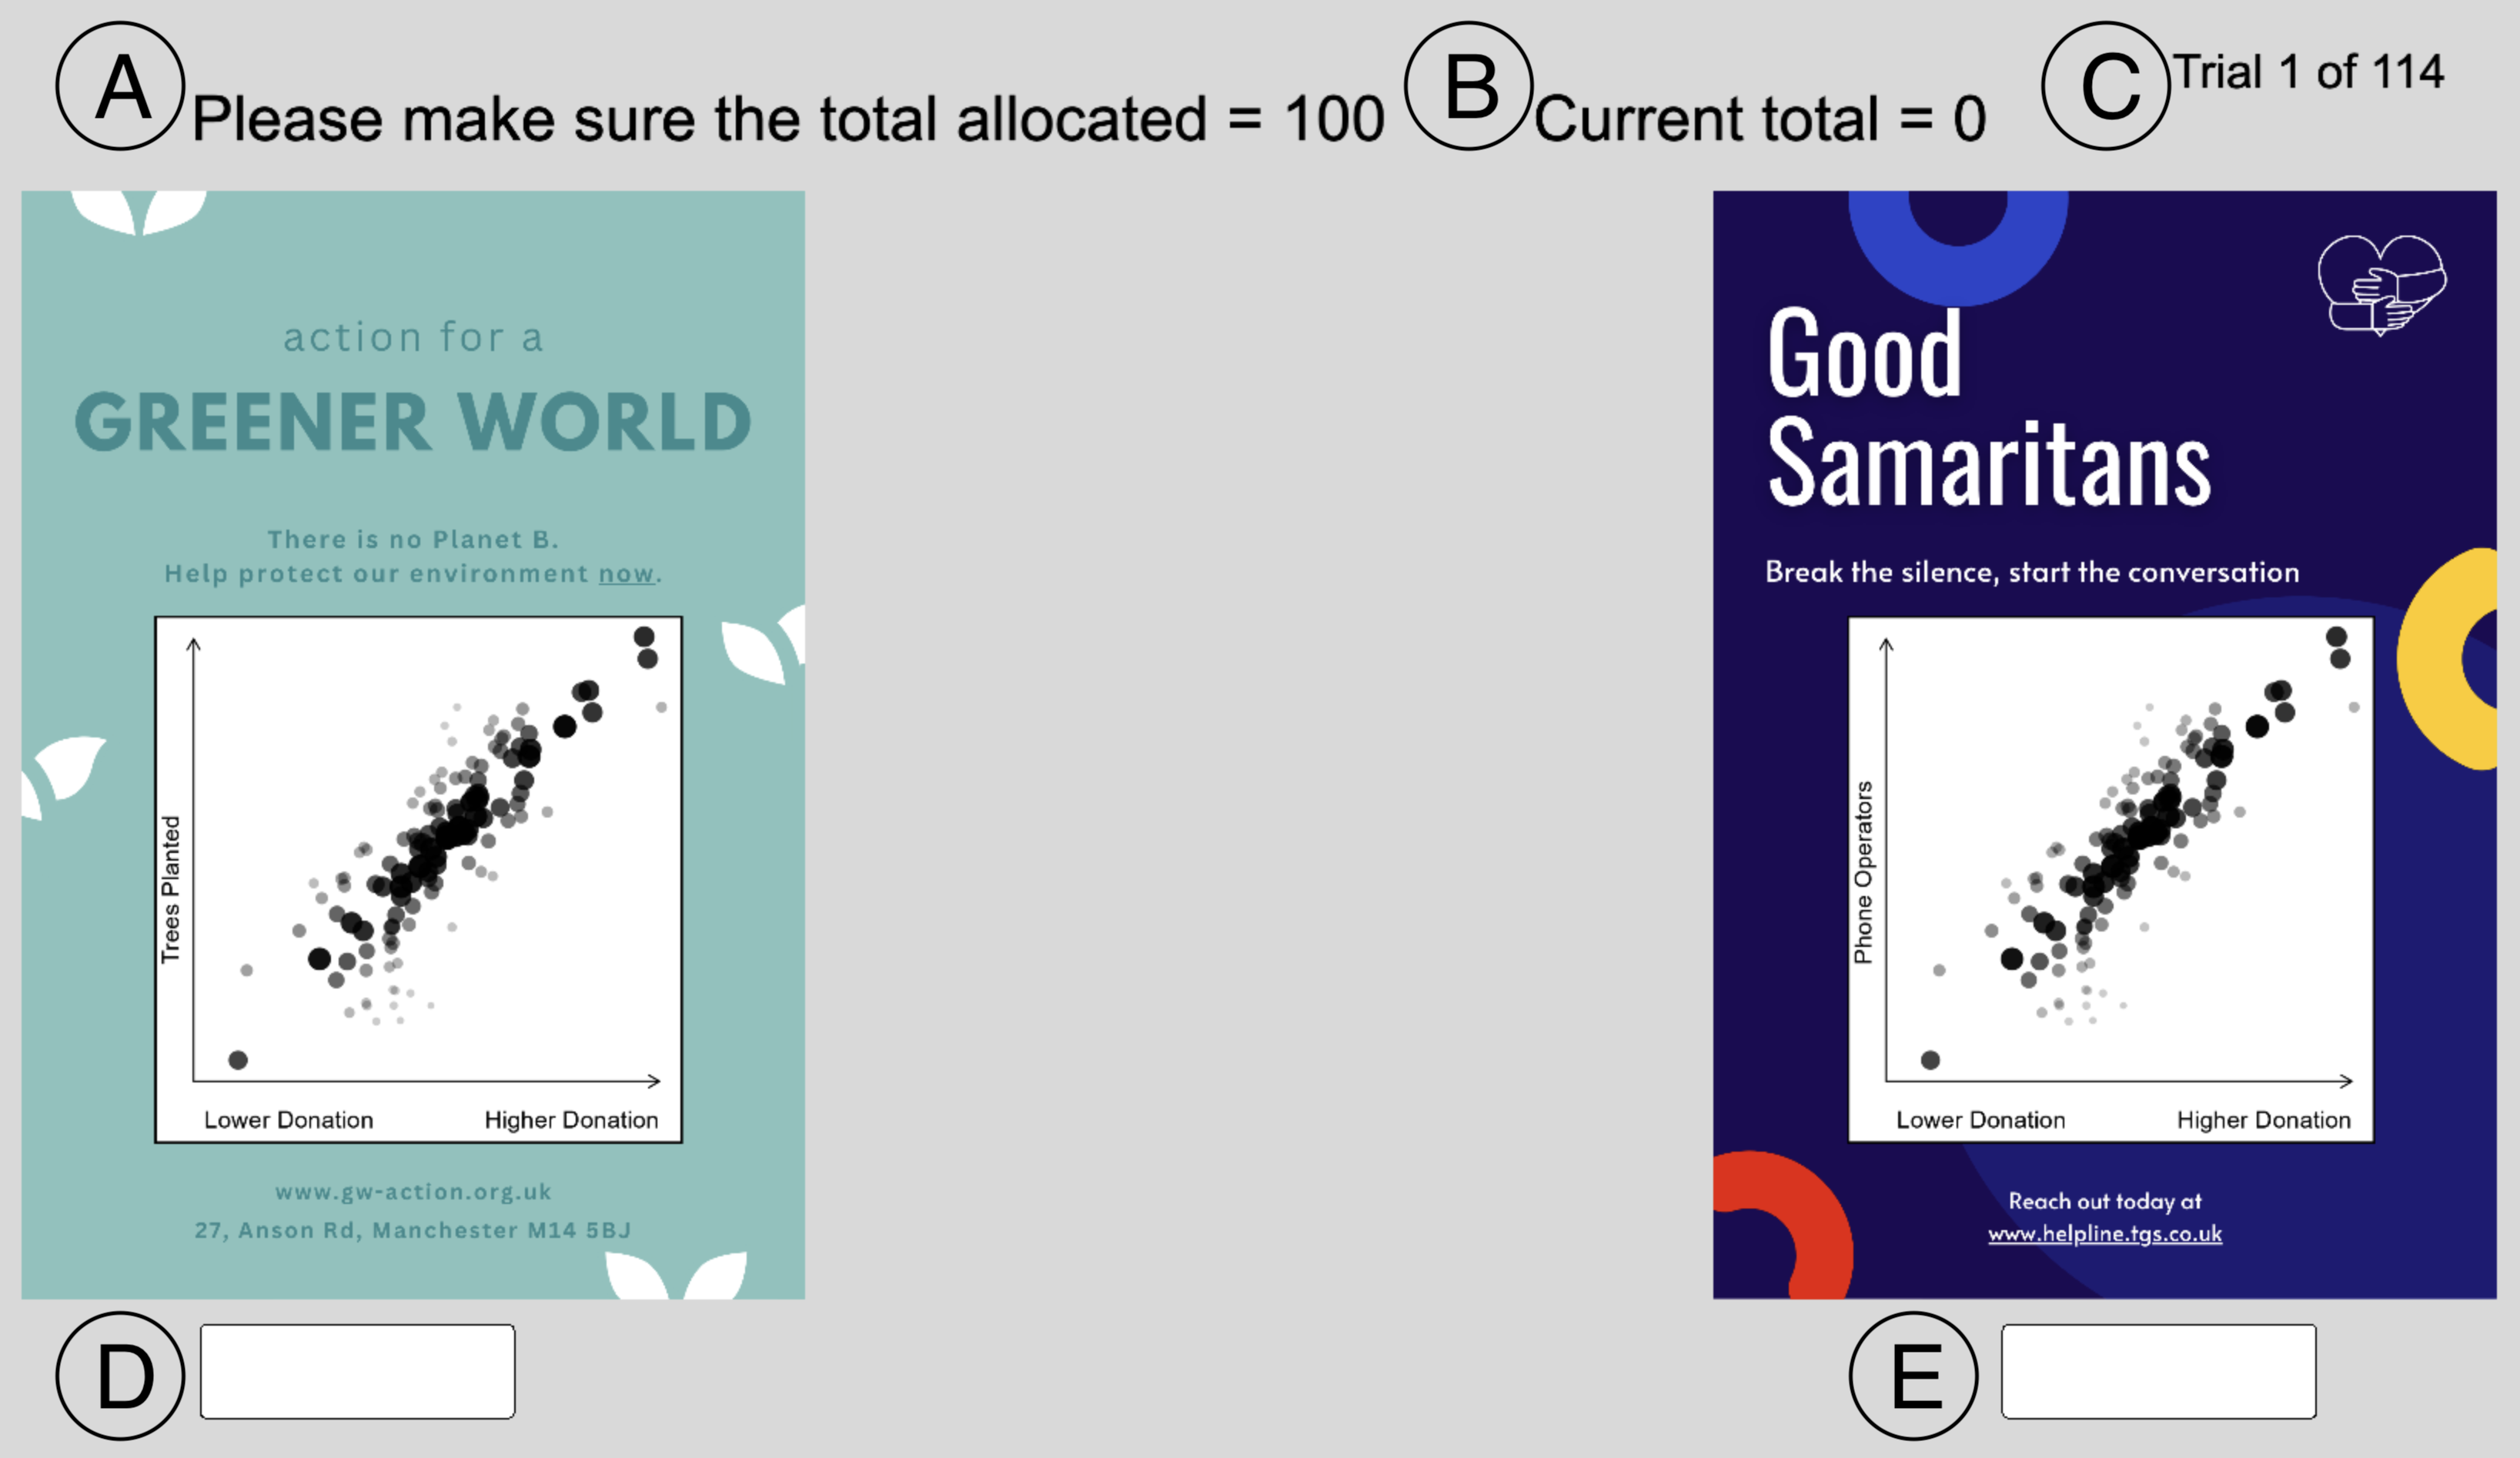
\includegraphics[width=1\linewidth,height=\textheight,keepaspectratio]{graphics/example_trial.png}

}

\caption{\label{fig-example-trial}An example of an experimental trial.
Illustrated are the reminder to use all available money (A), the display
of the current total (B), the trial counter (C), the left infographic
and allocation box (D), and the right infographic and allocation box
(E)}

\end{figure*}%

\subsection{Participants}\label{sec-participants}

Participants were recruited using Prolific \citep{prolific}. English
fluency and normal or corrected-to-normal vision were required, as well
as having not previously taken part in any of the research team's
previous studies into scatterplot visualisations (references withheld
for anon). In an effort to improve data quality, strict pre-screening
criteria were also employed \citep{peer_2021}; participants were
required to have previously completed at least 100 studies on the
platform, and were required to have been accepted on at least 99\% of
them. Data were collected from 174 participants. 10 failed more than 3
out of 6 attention checks, meaning their submissions were rejected in
accordance with our pre-registration
\href{The\%20pre-registration\%20states\%20that\%20150\%20participants\%20would\%20be\%20recruited.\%20Additional\%20participants\%20were\%20recruited\%20due\%20to\%20an\%20oversight,\%20however\%20all\%20conclusions\%20and\%20statistical\%20results\%20are\%20identical\%20when\%20run\%20with\%20164\%20or\%20150\%20participants.}{1\^{}}.
Data from the remaining 164 participants were included in the full
analysis (86 male, 76 female, and 2 non-binary). Participants' mean age
was 34.7 (SD = 11.2). Participants took a mean of 25.7 minutes to
complete the experiment (SD = 7.54).

\section{Results}\label{sec-results}

\section{Discussion}\label{sec-discussions}

\section{Conclusion}\label{sec-cocnlusion}

\bibliographystyle{ACM-Reference-Format}
\bibliography{donation-behaviour.bib}

%% begin pandoc before-bib
%% end pandoc before-bib
%% begin pandoc biblio
%% end pandoc biblio
%% begin pandoc include-after
%% end pandoc include-after
%% begin pandoc after-body
%% end pandoc after-body

\end{document}
\endinput
%%
%% End of file `sample-manuscript.tex'.
